\chapter{Evaluation Methodology}
\label{chap:evaluation-methodology}

This chapter describes the experimental setup used to evaluate \methodname{} and all compared methods. It covers the student models, benchmarks, training configuration, evaluation metrics and baselines. The ablation settings and implementation details needed to reproduce the main results are included at the end of the chapter.


\section{Experimental Setup}
All experiments follow a shared evaluation protocol for fair comparison across
methods. The experiments instantiate the student side with
\textbf{SmolVLM-500M} and \textbf{SmolVLM-256M}, evaluated on multimodal
benchmarks \cite{marafioti2025smolvlm}. All models are evaluated with
\textbf{VLM-Eval-Kit} \cite{duan2024vlmevalkit}, which provides a shared
inference, post-processing and metric-computation pipeline for the three
benchmarks. VLM-Eval-Kit uses a generation-based evaluation interface. For each benchmark
sample, the toolkit loads the image-question pair, applies the dataset-specific
prompt construction logic and calls the model's generation or chat interface to
produce a free-form text answer. This choice is important for VLMs because it
evaluates the same interface used at inference time and avoids replacing answer
generation with likelihood scoring over a fixed set of options. After
generation, the toolkit writes model predictions to result files and invokes
the benchmark-specific evaluator.

The post-processing stage depends on the task format. For structured
yes/no or multiple-choice tasks, VLM-Eval-Kit can use exact matching or an
LLM-based choice extractor to recover the final option from the generated text.
For open-answer VQA benchmarks such as the ones used here, the generated answer
is normalized before scoring so that superficial formatting differences do not
dominate the metric. The final score is then computed with the official metric
associated with each dataset. For example, a TextVQA prediction is matched
against the human answer set using VQA accuracy, so a short answer such as
\texttt{stop} is credited according to annotator agreement. A DocVQA prediction
is scored with ANLS, so a near miss such as \texttt{INV-4572} versus
\texttt{4572} receives partial credit only when the normalized edit similarity
is high enough. A ChartQA numeric answer is evaluated with relaxed accuracy, so
a value within 5\% of the reference number is counted as correct. In this
thesis, using the same toolkit for all methods fixes the prompt template,
decoding interface, answer normalization and metric implementation, so
evaluation-code differences do not drive the reported performance gaps.

\section{Datasets}
We evaluate three text-centric VQA benchmarks: \textbf{TextVQA}, \textbf{DocVQA} and \textbf{ChartQA}. These benchmarks test whether the model can read visual text, understand questions and perform basic reasoning across natural images, documents and charts. They were chosen because they cover complementary visual domains and combine OCR-heavy understanding with layout interpretation and numerical reasoning \cite{singh2019vqamodelsread,mathew2021docvqadatasetvqadocument,masry2022chartqabenchmarkquestionanswering}.

\textbf{TextVQA} tests question answering on natural images containing scene
text, requiring the model to read and reason over text embedded in real-world
scenes \cite{singh2019vqamodelsread}.
\textit{Sample question}: ``What word is written on the stop sign?''

\textbf{DocVQA} tests question answering on scanned document images, where
layout, paragraphs, tables and forms are central to answering correctly
\cite{mathew2021docvqadatasetvqadocument}.
\textit{Sample question}: ``What is the invoice number shown in this document?''

\textbf{ChartQA} tests question answering over charts, combining chart reading
with numerical and logical reasoning
\cite{masry2022chartqabenchmarkquestionanswering}.
\textit{Sample question}: ``Which year has the highest sales value in the chart?''

\stepcounter{footnote}
\begin{figure}
    \centering
    \begin{subfigure}{0.31\linewidth}
        \centering
        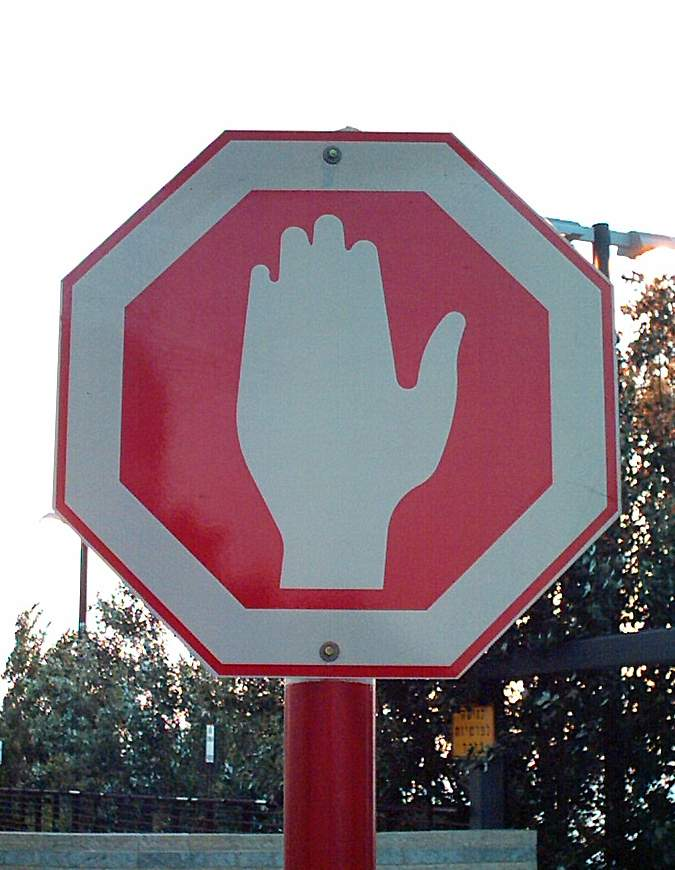
\includegraphics[width=\linewidth,height=0.18\textheight,keepaspectratio]{figures/textvqa_sample_stop_sign.jpg}
        \caption{TextVQA}
    \end{subfigure}
    \hfill
    \begin{subfigure}{0.31\linewidth}
        \centering
        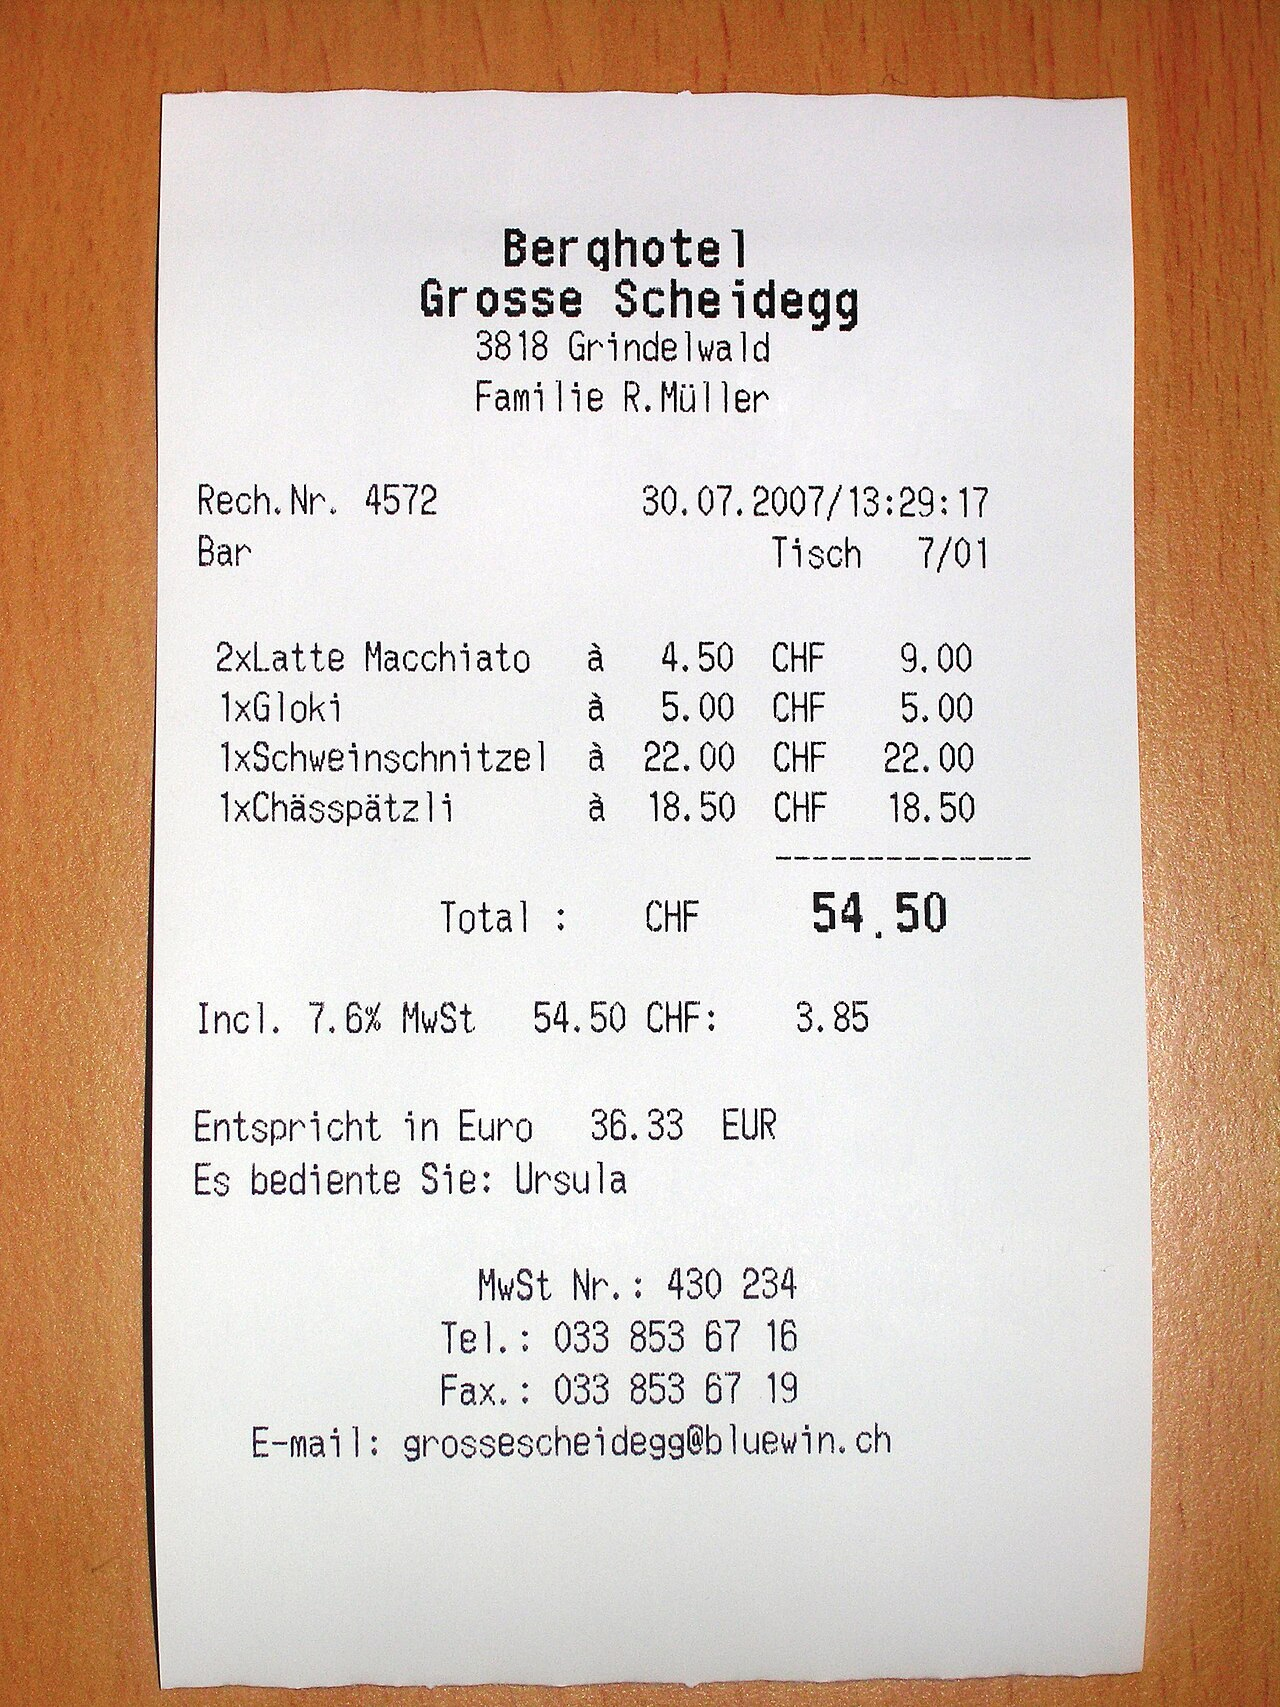
\includegraphics[width=\linewidth,height=0.18\textheight,keepaspectratio]{figures/docvqa_sample_receipt.jpg}
        \caption{DocVQA}
    \end{subfigure}
    \hfill
    \begin{subfigure}{0.31\linewidth}
        \centering
        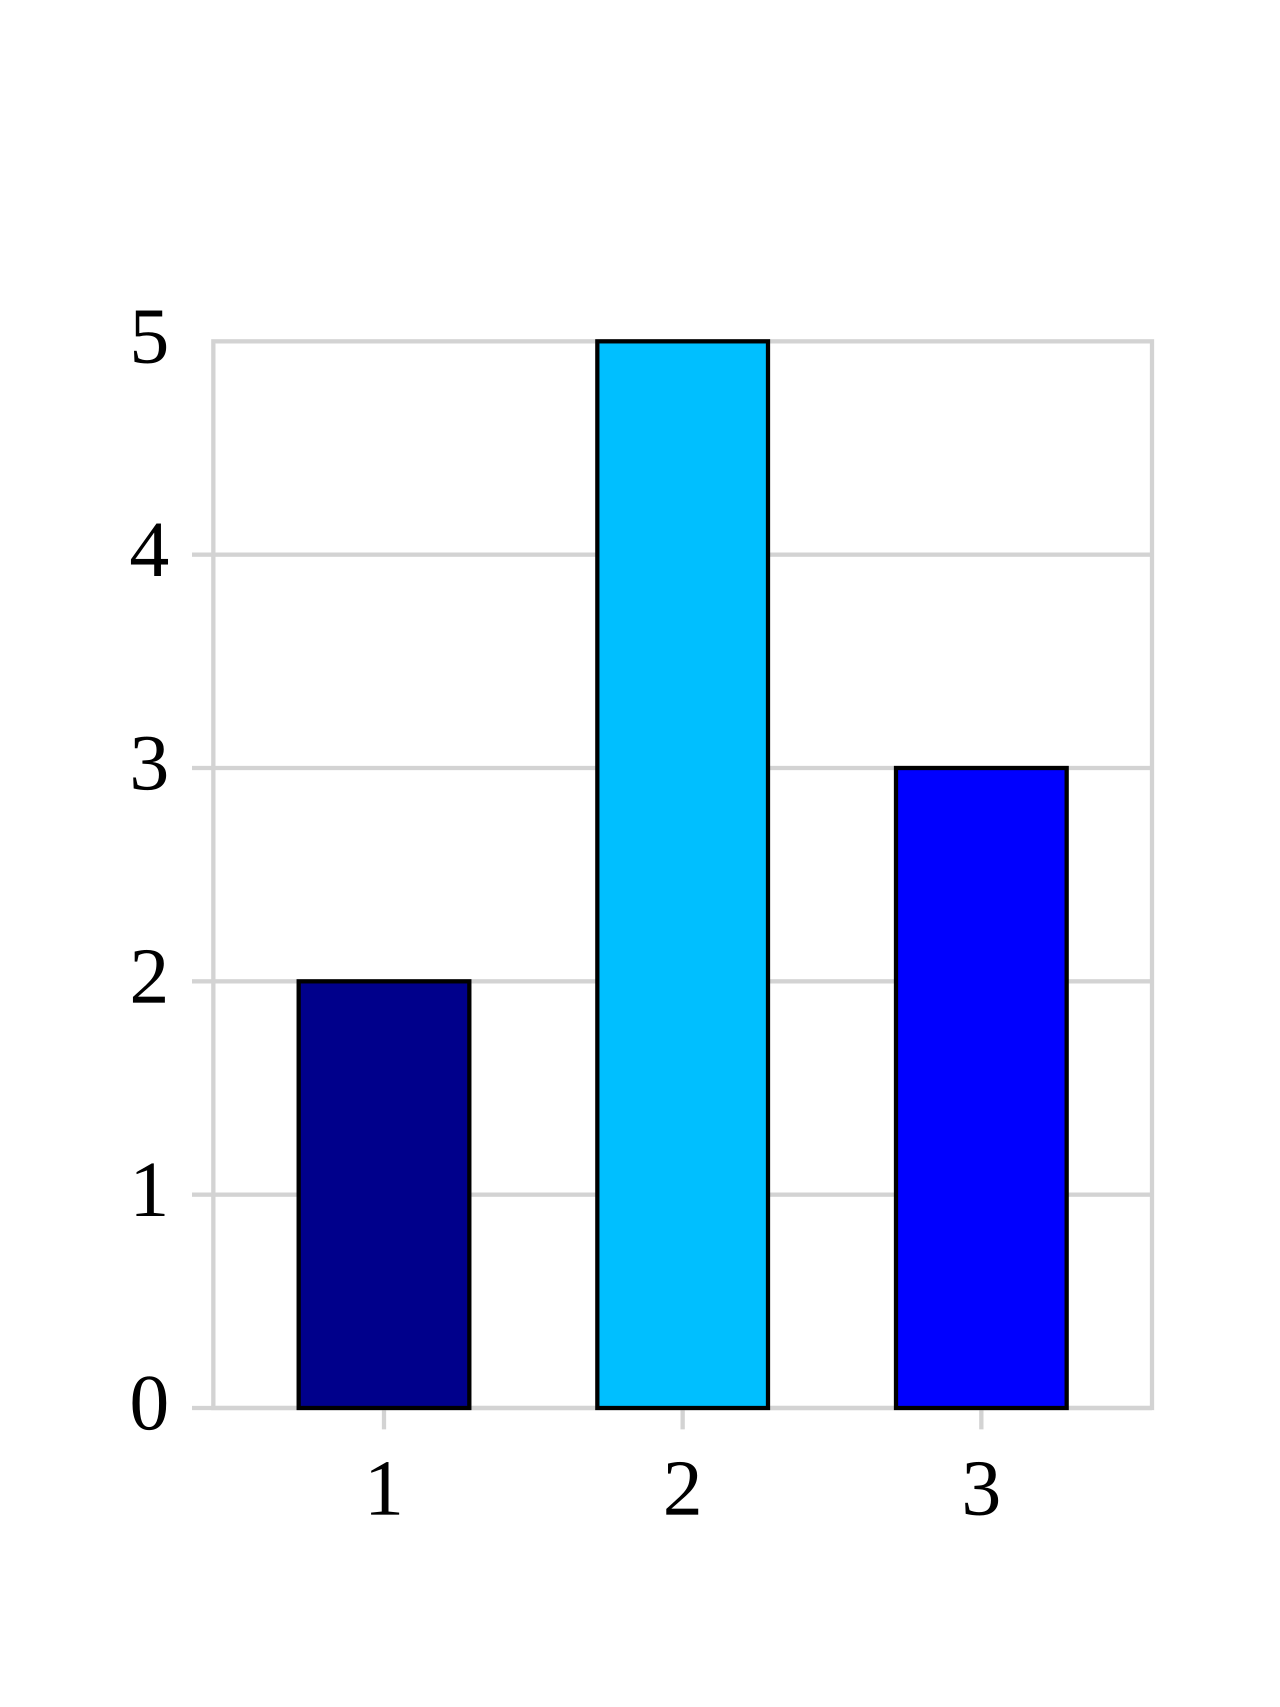
\includegraphics[width=\linewidth,height=0.18\textheight,keepaspectratio]{figures/chartqa_sample_bar_chart.png}
        \caption{ChartQA}
    \end{subfigure}
    \caption[Representative dataset examples.]{Representative dataset examples.\textsuperscript{\thefootnote}}
    \label{fig:dataset-samples}
\end{figure}
\footnotetext[\value{footnote}]{Images adapted from Wikimedia Commons sources~\cite{wikimedia_stop_sign_image,wikimedia_receipt_swiss_image,wikimedia_bar_chart_image}.}

Figure~\ref{fig:dataset-samples} shows the visual differences behind this
benchmark choice. The TextVQA panel represents natural-image reading, where the
relevant cue is embedded in an object in the scene. The DocVQA panel is a
receipt with fields, item rows and totals arranged by document layout. The
ChartQA panel is a bar chart, where answering requires comparing bar heights
and reading values from the plot structure. The evaluation therefore covers
natural scene text, document layouts and chart reasoning. The split sizes used
throughout the evaluation chapter are listed in Table~\ref{tab:dataset-sizes}.
\begin{table}[H]
\centering
\caption[Dataset split sizes.]{Dataset split sizes.}
\label{tab:dataset-sizes}
\scalebox{0.96}{
\begin{tabular}{lrrrr}
\toprule
\textbf{Dataset} & \textbf{Train} & \textbf{Val} & \textbf{Test} & \textbf{Total} \\
\midrule
TextVQA & 34,602 & 5,000 & 5,734 & 45,336 \\
DocVQA & 39,463 & 5,349 & 5,188 & 50,000 \\
ChartQA-H (human) & 7,398 & 960 & 1,250 & 9,608 \\
ChartQA-M (machine) & 20,901 & 960 & 1,250 & 23,111 \\
ChartQA (H+M, combined) & 28,299 & 1,920 & 2,500 & 32,719 \\
\bottomrule
\end{tabular}
}
\end{table}

\section{Training Configuration}

Before training, all benchmark samples are converted into a unified
\textbf{LLaVA-style multimodal instruction format}
\cite{liu2023visualinstructiontuning}. Each example is stored as an image plus
a short user-assistant dialogue, as shown in Listing~\ref{lst:llava-format},
so TextVQA, DocVQA and ChartQA can share the same data loader, prompt template
and answer supervision interface. This format is useful because the model sees
every task as the same conditional generation problem: given an image and a
natural-language user query, generate the assistant answer. It also separates
the visual input path from the textual instruction path while keeping the
answer span explicit, which makes it easier to mask prompt tokens, compute
supervised loss only on assistant tokens and align teacher logits with the same
answer positions during distillation.

\begin{lstlisting}[basicstyle=\ttfamily\footnotesize,breaklines=true,frame=single,caption={Representative LLaVA-style sample used after dataset conversion.},label={lst:llava-format}]
{
  "image": "sample_000123.jpg",
  "conversations": [
    {"from": "human", "value": "<image>\nWhat is the invoice number?"},
    {"from": "gpt", "value": "4572"}
  ]
}
\end{lstlisting}

We run all training jobs on a single high-memory \textbf{NVIDIA H200}
graphics processing unit (GPU) or on comparable single-GPU \textbf{Vast.ai}
instances, depending on availability.
Distillation training uses \textbf{DeepSpeed ZeRO Stage 2}, \textbf{Brain
Floating Point 16 (bf16)} mixed precision, \textbf{TensorFloat-32 (TF32)}
matrix multiplication and gradient checkpointing to control memory use while
keeping the student fully trainable and all teachers frozen
\cite{rajbhandari2020zero,chen2016sublinear}. Full optimization and routing
parameter values are reported in Appendix~\ref{app:experiment-parameters},
Table~\ref{tab:experiment-parameters}. Teacher-logit storage and remote caching
are documented in Appendix~\ref{app:offline-teacher-logit-preparation} and
Appendix~\ref{app:remote-logit-streaming} for reproducibility purposes.

\section{Evaluation Metrics}
We report benchmark-specific official metrics for each dataset.

\textbf{TextVQA.}
For TextVQA, we report the official VQA Accuracy metric. For a predicted
answer \(\hat{a}\), the per-question score is
\[
s_{\text{VQA}}=\min\left(\frac{\#\text{annotators that provided } \hat{a}}{3},\,1\right),
\]
and the final score is the mean over all questions \cite{singh2019vqamodelsread}.

\textbf{DocVQA.}
We report ANLS, the Average Normalized Levenshtein Similarity. The final ANLS
is the average score over all samples
\cite{mathew2021docvqadatasetvqadocument}:
\[
\mathrm{NLS}(a,\hat{a})=1-\frac{d_{\text{Lev}}(a,\hat{a})}{\max(|a|,|\hat{a}|)}, \quad
s_{\text{ANLS}}=
\begin{cases}
\mathrm{NLS}(a,\hat{a}), & \mathrm{NLS}\ge 0.5,\\
0, & \text{otherwise}.
\end{cases}
\]

\textbf{ChartQA.}
For ChartQA, we report Relaxed Accuracy \cite{masry2022chartqabenchmarkquestionanswering}.
A prediction is correct if it matches exactly for text answers. For numeric
answers, the score handles the zero-target case explicitly:
\[
s_{\mathrm{ChartQA}}=
\begin{cases}
\mathbf{1}[\hat{y}=y], & y=0,\\
\mathbf{1}\!\left[\frac{|\hat{y}-y|}{|y|}\le 0.05\right], & y\ne0.
\end{cases}
\]

\section{Baselines and Compared Methods}

For consistency with Chapter~\ref{chap:experiment-results}, we organize the
compared methods into four groups: non-distillation references, same-family
distillation baselines, different-family single-teacher baselines and
heterogeneous teacher baselines. Before introducing the method-specific baselines, the role of each baseline
family is grouped in Table~\ref{tab:baseline-groups}. The grouping separates
student-only references, same-family KD, tokenizer-mismatched single-teacher
transfer and heterogeneous teacher methods.

\begin{table}[tp]
\centering
\caption[Baseline groups.]{Baseline groups.}
\label{tab:baseline-groups}
\small
\setlength{\tabcolsep}{5pt}
\renewcommand{\arraystretch}{1.08}
\begin{tabular}{@{}
  >{\raggedright\arraybackslash}p{0.18\linewidth}
  >{\raggedright\arraybackslash}p{0.24\linewidth}
  >{\raggedright\arraybackslash}p{0.24\linewidth}
  >{\raggedright\arraybackslash}p{0.26\linewidth}@{}}
\toprule
\textbf{Group} & \textbf{Methods} & \textbf{Teacher setup} & \textbf{Purpose} \\
\midrule
Non-distillation references & Original, full finetuning & No teacher & Student-only reference points \\
\midrule
Same-family baselines & Forward KL, Reverse KL, Jensen-Shannon & SmolVLM2-2.2B-Instruct & Standard single-teacher objectives within the SmolVLM family \\
\midrule
Cross-family single-teacher & ULD & Qwen2-VL-2B-Instruct & Cross-family transfer without routed teacher selection \\
\midrule
Heterogeneous teacher baselines & Uniform averaging, SHM-CKA, REINFORCE, \textbf{\methodname{} (Ours)} & Mixed teacher set from multiple VLM families & Static averaging vs. hidden-state matching vs. adaptive teacher assignment \\
\bottomrule
\end{tabular}
\end{table}

The non-distillation references consist of the original student and the
full-finetuning baseline, which provide student-only reference points. The
same-family baselines use \textbf{SmolVLM2-2.2B-Instruct} as teacher for
forward KL, reverse KL and Jensen-Shannon distillation, isolating standard
teacher-student transfer when the tokenizer and output space are matched
\cite{smolvlm2_modelcard,marafioti2025smolvlm,hinton2015distillingknowledgeneuralnetwork,lin1991jensen,cui2024sinkhorn}.
The different-family single-teacher setting uses ULD with a teacher outside
the SmolVLM family, testing tokenizer-mismatched transfer without teacher routing
\cite{boizard2024towardscrosstokenizerdistillation}. The heterogeneous
teacher setting compares uniform averaging, SHM-CKA, REINFORCE and
\methodname{} over a mixed teacher pool, separating static averaging,
hidden-state matching and adaptive teacher assignment
\cite{takezawa2021supervisedtreewasserstein,zhang2023adaptivemultiteachermetalearning,yu2024selectdistill,dasgupta2025improving}.

For the trainable competitor methods, we keep the supervised term
\(\mathcal{L}_{CE}\). The logits-only baselines differ only in the KD signal,
but SHM-CKA also adds a hidden-state alignment term and REINFORCE
also adds a REINFORCE-style policy term
\cite{kornblith2019similarityrepresentations,williams1992simple,yuan2020reinforcedmultiteacherselection}.
In the descriptions below, \(\gamma\) denotes a generic KD mixing coefficient.
\(\alpha_{\mathrm{KD}}\) is reserved for the \methodname{} training objective
as defined in Equation~\ref{eq:final-objective}.

\textbf{Original.} Directly evaluates the released student without
additional optimization, thereby measuring the native capability of the student
model before task adaptation or any teacher-guided distillation signal.

\textbf{Full finetuning.} Optimizes only \(\mathcal{L}_{CE}\) and uses no teacher, which
isolates the effect of supervised task adaptation from any teacher-guided
distillation signal.

\textbf{Forward KL.} Uses
\(\mathcal{L}_{KD}=\mathrm{KL}(p_t\|p_s)\) for same-family soft-target
distillation when teacher and student vocabularies are aligned
\cite{hinton2015distillingknowledgeneuralnetwork}.

\textbf{Reverse KL.} Uses \(\mathcal{L}_{KD}=\mathrm{KL}(p_s\|p_t)\)
\cite{cui2024sinkhorn,wen2023fdistill} as a student-centered divergence
baseline, which tests whether matching the teacher from the student's current
distribution is suitable for VLM distillation. Because the reverse-KL gradient
is weighted by \(p_s\), this objective tends to emphasize regions where the
student already assigns probability.

\textbf{Jensen-Shannon.} Uses the symmetric divergence
\[
\frac{1}{2}\mathrm{KL}(p_s\|m)+\frac{1}{2}\mathrm{KL}(p_t\|m),
\qquad
m=\frac{1}{2}(p_s+p_t).
\]
It tests whether a bounded symmetric objective is more stable than KL
\cite{lin1991jensen,cui2024sinkhorn}.

\textbf{ULD.} Uses \(\mathcal{L}_{KD}=\|\pi(p_s)-\pi(p_t)\|_1\)
\cite{boizard2024towardscrosstokenizerdistillation}. This is the main
tokenizer-mismatched logits baseline because it compares ranked probability mass,
not token IDs.

\textbf{SHM-CKA.} Extends ULD with a hidden-state CKA penalty
\cite{boizard2024towardscrosstokenizerdistillation,dasgupta2025improving,kornblith2019similarityrepresentations}.
For the heterogeneous setting, both the ULD and layer-matching terms are
averaged uniformly across teachers before combining with \(\mathcal{L}_{CE}\).
Full implementation details are given in
Appendix~\ref{app:baseline-implementation-details}.

\textbf{Uniform multi-teacher.} Assigns fixed equal weights to all teachers
in the heterogeneous pool,
\(\mathcal{L}_{KD}=\frac{1}{M}\sum_{i=1}^{M}\mathcal{L}_{KD}^{(i)}\)
\cite{yuan2020reinforcedmultiteacherselection,zhang2023adaptivemultiteachermetalearning},
thereby testing whether teacher diversity alone is sufficient without adaptive
routing or gradient-aware weighting.

\textbf{REINFORCE.} Replaces deterministic routing with a stochastic policy
that samples teachers and updates the selector with REINFORCE
\cite{williams1992simple,yuan2020reinforcedmultiteacherselection}, providing
an adaptive routing baseline that does not use the gradient-agreement
refinement introduced by \methodname{}.
The selector is trained with the policy-gradient term
\begin{equation}
\mathcal{L}_{\mathrm{pol}}
=
-(r-b)\log p(\mathbf{m}\mid\boldsymbol{\pi}),
\end{equation}
where \(r\) is the reward, \(b\) is an EMA reward baseline and
\(\mathbf{m}\) is the sampled teacher mask. Its final training objective is
\begin{equation}
\mathcal{L}_{\mathrm{RS}}
=
\mathcal{L}_{CE}
+ \gamma \mathcal{L}_{KD}
+ \lambda_{\pi}\mathcal{L}_{\mathrm{pol}}.
\end{equation}
Additional baseline implementation details are reported in
Appendix~\ref{app:baseline-implementation-details}.


\section{Ablation Settings}
\label{sec:ablation-settings}

The ablation study in Section~\ref{sec:ablation} isolates the main components
of \methodname{} on DocVQA while keeping the teacher set and training protocol
close to the final method. The variants change one mechanism at a time so that
the result table can separate teacher diversity, sparse routing,
gradient-agreement weighting and EMA score smoothing.
The effect of EMA smoothing is isolated in the \(\beta_{\mathrm{EMA}}=0\)
ablation in Section~\ref{sec:ablation}.

\textbf{Cross-family ULD.} The single-teacher cross-family baseline uses one teacher outside the SmolVLM
family and optimizes
\[
\mathcal{L}
=
\mathcal{L}_{CE}
+
\alpha_{\mathrm{KD}}\mathcal{L}_{ULD},
\qquad
\mathcal{L}_{ULD}
=
\|\pi(p_s)-\pi(p_t)\|_1 .
\]

\textbf{Uniform averaging.} The uniform variant adds the full heterogeneous teacher pool but assigns fixed
equal weights:
\[
\mathcal{L}
=
\mathcal{L}_{CE}
+
\alpha_{\mathrm{KD}}\frac{1}{M}\sum_{i=1}^{M}\mathcal{L}_{TW}^{(i)}.
\]
This setting tests whether teacher diversity alone is enough without adaptive
selection.

\textbf{Routing only.} The routing-only variant keeps sparse teacher selection but replaces
post-routing weights with uniform weights within the routed set:
\[
w_i^{(b)}
=
u_i^{(b)}
=
\frac{\mathbf{1}[i\in\mathcal{R}_b]}{|\mathcal{R}_b|}.
\]
This setting tests whether top-\(k\) routing is useful without
gradient-agreement refinement.

\textbf{Full GRACE.} The full method combines trie-Wasserstein KD, sparse routing and
gradient-agreement weighting:
\[
w_i^{(b)}
\propto
(\hat p_i^{(b)})^{\lambda_{\mathrm{blend}}}
(\omega_i^{(b)})^{1-\lambda_{\mathrm{blend}}}.
\]
Two additional ablation variants isolate the final weighting mechanism,
reported in Table~\ref{tab:docvqa-planned-ablation}. The
\(\lambda_{\mathrm{blend}}=1.0\) variant keeps the active-set threshold and
fallback rules but removes the score-softmax factor from the confident-score
case:
\[
w_i^{(b)}
\propto
\hat{p}_i^{(b)}\mathbf{1}[i\in\mathcal{A}_b].
\]
This row is an active-set-restricted router-weight ablation, not a pure
router-only ablation over all routed teachers. The \(\beta_{\mathrm{EMA}}=0\)
variant removes temporal smoothing by setting \(\hat{s}_i=s_i\) before
score-softmax weighting.

The training runs reported in this thesis rely on an offline teacher-logit
preparation step and a remote logit-streaming infrastructure that are
separate from the fair-comparison protocol described above. Teacher logits are
generated once and stored on Cloudflare R2. During training, they are streamed
lazily through a 100~GB local cache without copying the full logit store locally.
Full engineering
details, including the caching script, path conventions, streaming loader and
the logit-streaming settings table, are given in
Appendix~\ref{app:offline-teacher-logit-preparation} and
Appendix~\ref{app:remote-logit-streaming}.
